\documentclass[12pt]{article}


%%%%% Preamble

%% Packages to use

\usepackage{amsmath,amsfonts,amssymb}   %% AMS mathematics macros
\usepackage{physics}
\usepackage{setspace}
\usepackage{cite}
\usepackage{siunitx}
\usepackage{graphicx}
\usepackage{xcolor}


% MARKUPS
\newcommand{\cmt}[1]{{\color{orange}{(#1)}}}
\newcommand{\todo}[1]{{\color{red}{(#1)}}}
\newcommand{\question}[1]{{\color{magenta}{(#1)}}}
\newcommand{\comment}[1]{{\color{green!70!black}{(#1)}}}
\newcommand{\note}[1]{{\color{cyan}{(#1)}}}

%% Title Information.

\title{System Of ODE solver and the Two Body Problem}
\author{Craig Tenney}
%% \date{2 July 2004}           %% By default, LaTeX uses the current date

%%%%% The Document



\begin{document}
\maketitle

\section{Background}

With two bodies interacting with only the force of gravity, we only have one force acting on each body

\begin{equation}
\begin{aligned}
&F_1 = -Gm_1m_2 \frac{(x_1-x_2)}{\abs{x_1-x_2}^3}\\
\\
&F_2 = -Gm_1m_2 \frac{(x_2-x_1)}{\abs{x_2-x_1}^3}
\end{aligned}
\end{equation} 
%
where $G$ is Newton's gravitational constant, $m_1$ and $m_2$ are the masses of the bodies, and $x_1$ and $x_2$ are the positions. We can use Newtons 2nd Law

\begin{equation}
F = ma = m \ddot{x}
\end{equation}
%
and rewrite the force equations into two 2nd order differential equations 
 
\begin{equation}
\begin{aligned}
    &\ddot{x_1} = -Gm_2 \frac{(x_1-x_2)}{\abs{x_1-x_2}^3}\\
    \\
    &\ddot{x_2} = -Gm_1 \frac{(x_2-x_1)}{\abs{x_2-x_1}^3}
\end{aligned}
\end{equation}
%
by a change of variable $Y = \mqty[x_1  \\ x_2 \\ \dot{x_1} \\ \dot{x_2}]$ we can convert the 2nd order equations to a system of four first order equations:

\begin{equation}
\begin{aligned}
&\dot{Y_1} = Y_3\\
\\
&\dot{Y_2} = Y_4\\
\\
&\dot{Y_3} = -Gm_2 \frac{(Y_1-Y_2)}{\abs{Y_1-Y_2}^3}\\
\\
&\dot{Y_4} = -Gm_1 \frac{(Y_2-Y_1)}{\abs{Y_2-Y_1}^3}\\
\end{aligned}
\end{equation}

Now these equations can be sovled by a system of ODE solver.

\section{Computational Details}

We can employ the Runge-Kutta Method for Systems of Differential Equations, Chapter 5.9 Algorithm 5.7.

The system method is based off of the 1D Runge-Kutta method of order four:

\begin{equation}
\begin{aligned}
&\omega_0 = \alpha\\
\\
&k_1 = hf(t_i,\omega_i)\\
\\
&k_2 = hf(t_i + \frac{h}{2},\omega_i + \frac{1}{2}k_1)\\
\\
&k_3 = hf(t_i + \frac{h}{2},\omega_i + \frac{1}{2}k_2)\\
\\
&k_4 = hf(t_i,\omega_i+k_3)\\
\\
&\omega_{i+1} = \omega_i + \frac{1}{6}(k_1+2k_2+2k_3+k_4)\\
\end{aligned}
\end{equation}

To apply this to a system of equations, we just turn $f$, $w$, $t$, and $k_{1-4}$ into column vectors.
Then we can loop over each discretized increment of time, solve for $\omega_{i+1}$ and store the solution in a vector.
Once the iterations are finished, the program outputs the solution vector and the time vector. 


\section{Results}

As a test problem, we solved problem 5.9: 1c. and got
\\
\\
$
\begin{array}{lll}
 \omega_1   &     \omega_2& \omega_3 \\
 1.         &         0.  &      1.         \\
 0.70787076 & -1.24988663 &  0.39884862 \\
-0.33691753 & -3.01764179 & -0.29932294 \\
-2.41332734 & -5.40523279 & -0.92346873 \\
\end{array}  
$
\\
\\
as the solution, which matches the solution in the back of the book. 
 
Now we can look at solution to the two body problem. As an input we have to provide initial position and velocity of the bodies. We are able to set the mass and gravitational constant to our liking in arbitrary units. Then the solver will out put a vector of its position and velocity of time, so we are able to plot its trajectory. 

For $G=1$, $m_1 = 1$, $m_2 = 1000$, and 

$
\begin{array}{ll}
& x_1 = (0.0, 0.0)\\
& x_2 = (0.0, 10.0)\\
& v_1 = (9.0, 9.0)\\
& v_2 = (0.5, 0.0),
\end{array}
$
\\
mass 2 is much greater then mass 1 and has an initial slow velocity in the x direction. Body 2 is given a large xy velocity kick. And we get the following solution:

\begin{figure}[h!]
    \centering
    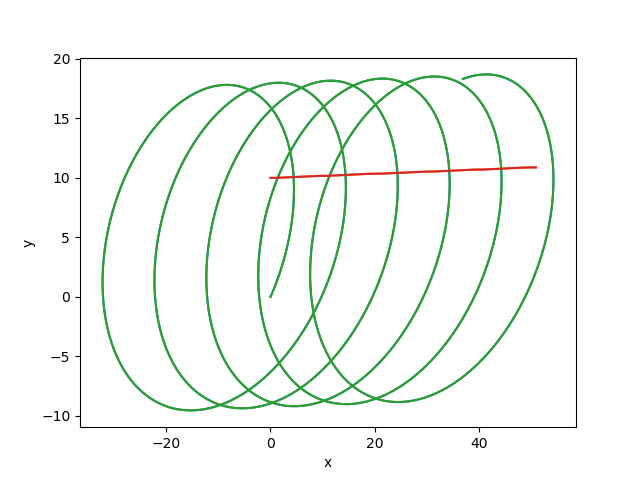
\includegraphics[scale=0.6]{1.png}
    %\caption{Experimental/theoretical Phase diagram of hydrogen \cite{dias2017observation}. } 
    \label{fig:1}
\end{figure}
and we can see body 1 (red) has only little deviation from its initial +x trajectory. Body 2 (green) is seen orbiting body 1.

Many different scenarios are possible with different initial conditions, and values of mass.

As another check on the ode solver, it was compared to the inbuilt python ode solver, odeint. The error between the ode solver and odeint for some of the positions are: 0.00000000e+00 ,1.18365107e-09,   2.21729754e-09 ..., 9.87021704e-04, 9.86631272e-04, 9.86241103e-04. So not terrible. One downside to our ode solver is the runtime is considerably longer then ondeint. 

\end{document}

